\documentclass{scrartcl}
\usepackage[utf8]{inputenc}
\usepackage[english]{babel}
\usepackage{caption}
\usepackage{subcaption}
\usepackage{listings}
\usepackage{pdfpages}
\usepackage{amsmath,amssymb}
\usepackage{siunitx}
\usepackage{hyperref}
\usepackage{mhchem}
\usepackage[section]{placeins}
\usepackage[activate, protrusion=true, expansion=true]{microtype}
\usepackage[left=2.5cm, right=2.5cm, bottom=2.5cm, top=2.5cm]{geometry}
\usepackage{libertine}
\usepackage{longtable}

\newcommand{\qed}{\hfill $\blacksquare$}
\newcommand{\gitlab}{\href{https://gitlab.lrz.de/arne/neuroprosthetics}{GitLab}}
\newcommand{\bb}[1]{\boldsymbol{#1}}

\lstset{frame=single,keepspaces=true,captionpos=b}

\title{Case Study:\\Path Tracking for an Autonomous Vehicle}
\subtitle{Multivariate Control and Coordination Systems (EE-477)}
\author{\textsc{Arne Sachtler}}
\date{Lausanne, EPFL, 2018}

\begin{document}
\maketitle
\tableofcontents

\setcounter{section}{-1}
\section{Introduction}
The general objective of the case study is to follow a trajectory with the vehicle.
Trajectories are expressed in a parametric form, where a parameter $s$ specifies the displacement of the car on the trajectory.
Figure~\ref{fig:vehicle_model} shows the model and important parameters.
\begin{figure}[h]
	\centering
	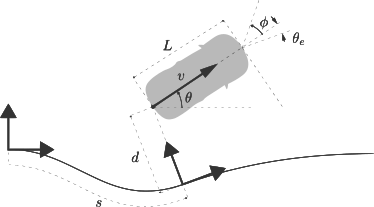
\includegraphics[width=.6\textwidth]{figures/model.pdf}
	\caption{Model of trajectories and the vehicle. Taken from the case study handout.}
	\label{fig:vehicle_model}
\end{figure}
For the dynamic equations several symbols are used. 
Table~\ref{tab:symbols} shows a summary of the symbols used within the document.
\begin{table}[h]
	\centering
	\begin{tabular}{c|l}
	\hline
	\hline
	\textbf{Symbol} & \textbf{Decription}\\
	\hline
		 $s$ & curvilinear coordinate\\
		 $d$ & lateral deviation between vehicle and path\\
		 $\theta_e$ & heading error\\
		 $v$ & longitudinal speed\\
		 $L$ & car length\\
		 $\phi$ & steering wheel angle\\
		 $\alpha$ & speed reference\\
		 $\beta$ & steering wheel angle reference\\
		 $\sigma_a, \sigma_s$ & dynamics of the actuators\\
		 $\kappa(s)$ & curvature of path at position s\\
	\hline
	\hline
	\end{tabular}
	\caption{Symbols used in the dynamics model of the vehicle}
	\label{tab:symbols}
\end{table}

\subsection*{State space model of the Vehicle}
The vehicle is modelled using a set of nonlinear differential equations in state space representation $\mathbf{\dot{x}} = \mathbf{f}(\mathbf{x}, \mathbf{u}, t)$.
The state vector of the system is defines as
\begin{equation}
	\mathbf{x} = \begin{bmatrix}
		x_1, &x_2, &x_3, &x_4, &x_5
	\end{bmatrix} = \begin{bmatrix}
		s, &d, &\theta_e, &v, &\phi
	\end{bmatrix}\, ,
\end{equation}
and the input
\begin{equation}
	\mathbf{u} = \begin{bmatrix}
		u_1, &u_2	
	\end{bmatrix} = \begin{bmatrix}
		\alpha, &\beta
	\end{bmatrix}\, .
\end{equation}
The model of the vehicle is provided in the case study handout
\begin{eqnarray}
	\dot{x_1} &=& \frac{x_4 \cos(x_3)}{1 - x_2\kappa}\label{eq:ss1}\\
	\dot{x_2} &=& x_4 \sin(x_3)\label{eq:ss2}\\
	\dot{x_3} &=& \frac{x_4}{L}\tan(x_5) - \frac{\kappa x_4 \cos(x_3)}{1 - x_2 \kappa}\label{eq:ss3}\\
	\dot{x_4} &=& \sigma_a (u_1 - x_4)\label{eq:ss4}\\
	\dot{x_5} &=& \sigma_s (u_2 - x_5)\label{eq:ss5}
\end{eqnarray}
For the time being, the state vector is also the output of the model.
\section{Linearization, Discretization and Simulation}
In this first part of the case study. The given system model of the path tracking system is analyzed and simulated.
Therefore, the system will be linearized and discretized. 
As a nominal trajectory is required for the linearization, these will be computed first.
In the end of this first part, simulation results of the simulated non-linear system, the linearized system and a dicretized linear system will be compared.

\subsection{Nominal Trajectories}
First, a nominal trajectory is computed.
A nominal trajectory is a function of the state variables and the input variable of time.
The nominal trajectories are a solution of the system model.

In order to obtain a nominal trajectory some contraintes are added to the state space equations.
It is assumed that the vehicle perfectly follows the desired trajectory.
Therefore, the lateral deviation and the heading error are zero and stay zero among all times.
Further, a constant speed is assumed.
Using these assumptions several contraints are added to the state space model.
Table~\ref{tab:nominal_contraints} summarizes the constraints.
\begin{table}[h]
	\centering
	\begin{tabular}{c|l}
	\hline
	\hline
	\textbf{Constraint} & \textbf{Description}\\
	\hline
	$\bar{x}_2 = 0$\\$\bar{\dot{x}}_2 = 0$ & no lateral deviation\\\hline
	$\bar{x}_3 = 0$\\$\bar{\dot{x}}_3 = 0$& no heading error\\\hline
	$\bar{x}_4 = v_{ref}$\\$\bar{\dot{x}}_4 = 0$& constant speed\\\hline
	$\bar{\dot{x}}_5 = 0$ & steering wheel actuator is at steady state\\
	\hline
	\end{tabular}
	\caption{Contraints for the nominal trajectory.}
	\label{tab:nominal_contraints}
\end{table}

\noindent Using \eqref{eq:ss1} we obtain
\begin{equation}
	\bar{\dot{x}}_1 = v_{ref} \Rightarrow \bar{x}_1 = v_{ref} \cdot t
\end{equation}
and using \eqref{eq:ss3}
\begin{equation}
	0 = \frac{v_{ref}}{L} \tan(\bar{x}_5) - \kappa v_{ref} \Rightarrow \bar{x}_5 = \arctan (\kappa L) \, .
\end{equation}
Further, using the actuator equations \eqref{eq:ss4} and \eqref{eq:ss5} the control input can be computed.
Finally, the resulting nominal trajectory for the state $\bar{x}$ is
\begin{eqnarray}
	\bar{x}_1 &=& v_{ref} \cdot t\\
	\bar{x}_2 &=& 0\\
	\bar{x}_3 &=& 0\\
	\bar{x}_4 &=& v_{ref}\\
	\bar{x}_5 &=& \arctan (\kappa L)
\end{eqnarray}
and for the control input $\bar{u}$
\begin{eqnarray}
	\bar{u}_1 &=& v_{ref}\\
	\bar{u}_2 &=& \arctan (\kappa L)\, .
\end{eqnarray}

\subsection{Linearization using Small Signal Linearization}
For the linearization of the system the small signal linearization approximation for deviations close to the nominal trajectory are used.
Therefore, Jacobians of the system model $\mathbf{\dot{x}} = \mathbf{f}(\mathbf{x}, \mathbf{u}, t)$ with respect to the state vector $\mathbf{x}$ and the input vector $\mathbf{u}$ are computed.
First the Jacobian of the nonlinear system model with respect to the state is computed
\begin{equation}
	\frac{\partial \mathbf{f}}{\partial \mathbf{x}} = \begin{bmatrix}
		0 & \frac{\kappa x_4 \cos(x_3)}{(kx_2 - 1)^2} & -\frac{x_4 \sin (x_3)}{1 - x_2 \kappa} & \frac{\cos (x_3)}{1 - x_2 \kappa} & 0\\
		0 & 0 & x_4 \cos(x_3) & \sin(x_3) & 0\\
		0 & -\frac{\kappa^2 x_4 \cos(x_3)}{(\kappa x_2 - 1)^2} & \left(\frac{1}{L}\tan(x_5) - \frac{\kappa \cos (x_3)}{1 - x_2 \kappa}\right) & \frac{\kappa x_4 \sin(x_3)}{1 - x_2 \kappa} & \frac{x_4}{L \cos^2(x_5)}\\
		0 & 0 & 0 & -\sigma_a & 0\\
		0 & 0 & 0 & 0& -\sigma_s\\
	\end{bmatrix}
\end{equation}
and the Jacobian with respect to the input is
\begin{equation}
	\frac{\partial \mathbf{f}}{\partial \mathbf{u}} = \begin{bmatrix}
		0 & 0\\
		0 & 0\\
		0 & 0\\
		\sigma_a & 0\\
		0 & \sigma_s
	\end{bmatrix}\, .
\end{equation}
In the small signal linearization technique the system is linearized around the nominal trajectory.
Therefore, the system is transformed to the nominal trajectory using
\begin{equation}
	\boldsymbol{\tilde{x}} = \mathbf{x} - \boldsymbol{\bar{x}}
\end{equation}
and
\begin{equation}
	\boldsymbol{\tilde{u}} = \mathbf{u} - \boldsymbol{\bar{u}} \, .
\end{equation}
Using the identity $\arctan(x) = \frac{1}{1 + x^2}$ the dynamics of the deviation from the nominal trajectory are now approximated by the linear model and the Jacobian is computed at the nominal trajectory
\begin{equation}
	\bb{\dot{\tilde{x}}} = \mathbf{A}\bb{\tilde{x}} + \mathbf{B}\bb{\tilde{u}} = \begin{bmatrix}
		0 & \kappa v_{ref} & 0 & 1 & 0\\
		0 & 0 & v_{ref} & 0 & 0\\
		0 & -\kappa^2 v_{ref} & 0 & 0 & \frac{v_{ref}}{L} \left(1 + L^2 \kappa^2\right)\\
		0 & 0 & 0 & -\sigma_a & 0\\
		0 & 0 & 0 & 0 & -\sigma_s
	\end{bmatrix} \bb{\tilde{x}} + \begin{bmatrix}
		0&0\\
		0&0\\
		0&0\\
		\sigma_a & 0\\
		0 & \sigma_s
	\end{bmatrix} \bb{\tilde{u}}
\end{equation}
and
\begin{equation}
	\bb{\tilde{y}} = \mathbf{C}\bb{\tilde{x}} + \mathbf{D}\bb{\tilde{u}} = \mathbf{I}\bb{\tilde{x}}\, .
\end{equation}

\subsection{Discretization}
TODO:
\begin{itemize}
	\item Euler
	\item $\Psi$
	\item MATLAB
\end{itemize}

\subsection{Simulation}
All three models, namely
\begin{itemize}
	\item the nonlinear, continuous-time model,
	\item the linearized continuous-time model and
	\item the linearized discrete-time model
\end{itemize}
are implemented in SIMULINK based on the template provided. 
Figure~\ref{fig:simu_simulink} shows the complete diagram.
Further, the nonlinear model block is completed based on equations \eqref{eq:ss1} to \eqref{eq:ss5}.
For the simulation the paramters are set to the values given in Table~\ref{tab:simu_param_values}.

\begin{figure}[h]
	\centering
	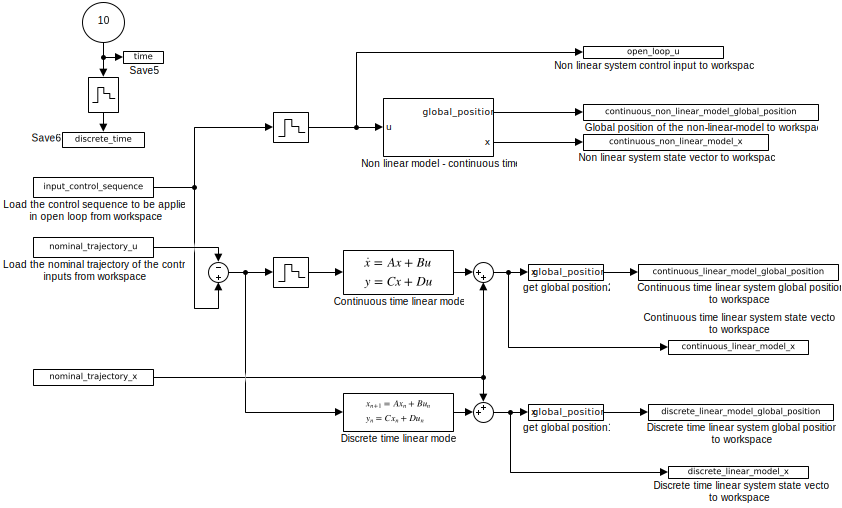
\includegraphics[width=\textwidth]{figures/simu_model.pdf}
	\caption{Simulink model for the simulation}
	\label{fig:simu_simulink}
\end{figure}

\begin{table}[h]
	\centering
	\begin{tabular}{c|l}
	\hline
	\hline
	\textbf{Parameter} & \textbf{Value}\\
	\hline
	$L$ & $4$\\
	$\kappa (s)$ & $1e^{-10}$\\
	$\sigma_a$ & 5\\
	$\sigma_s$ & 1\\
	$v_{ref}$ & 3\\
	\hline
	\hline
	\end{tabular}
	\caption{Values for the system parameters used in the simulation}
	\label{tab:simu_param_values}
\end{table}
In order to investigate the behaviour of the systems, several experiments are carried out on the model.
Among all simulation the initial condition $\bb{x}_0$ is set to the initial value of the nominal trajectory 
\begin{equation}
	\bb{x}_0 = \bb{\bar{x}} (0) \, 
\end{equation}
and the system has no transience at $t = 0$. 
The initial state for the linearized systems $\bb{\tilde{x}}_0$ is always set to $0$ such that, again, the system has no transience at $t=0$.
Below, different simulations and experiments on the system are presented.

\paragraph{Exact Model in the Linear Subspace of the System: }
Consider again the system model $\mathbf{\dot{x}} = \mathbf{f}(\mathbf{x}, \mathbf{u}, t)$ in equations \eqref{eq:ss1} to \eqref{eq:ss5}.
The system is linear, as long as all the quantities ($x_2$, $x_3$ and $x_5$) stay constant, there is no heading error $x_3 = 0$ and the curvature $\kappa$ is zero.
In this case, the trigonimetric functions in the differential equations behave as constants and the $\frac{1}{1- \kappa x_2}$ terms vanish.
On the nominal trajectory is no heading error and the curvature is very close ($\kappa = 1e^{-10}$) to zero.
Therefore, in this case, even the nonlinear system model behaves linearly.
The expectation is that there should be approximately no linearization error when applying $\bb{\bar{u}}$ as $\kappa$ is very small.
The same is true, when applying a varying reference speed as control input $u_1$ as long as the curvature is approximately zero and there is no error.
Figure~\ref{fig:ex1_ex2} shows two experiments, where the system is kept in the linear regime.
On the left, exactly the nominal input is applied as control input.
On the right, a step is applied in the reference velocity control signal $u_1$.
As the curvature is very small, the angular quantities are zero and the lateral error is zero, the system behaves approximately linearly and therefore the linearized models predict the system very well.
Even though, the step is rather large (from $3$ to $60$) the linearized systems show a good prediction of the states.
There are only very small errors in the angular state less than $2\cdot 10^{-8}$.


\begin{figure}[h]
	\centering
	\begin{subfigure}{0.49\textwidth}
	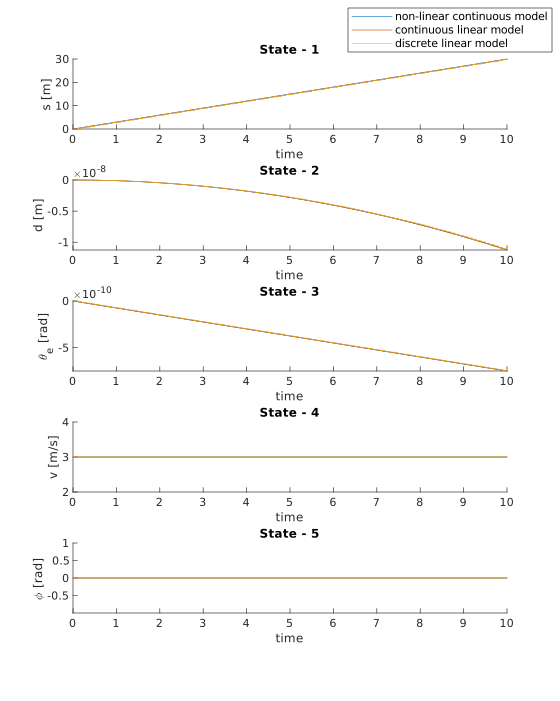
\includegraphics[width=\textwidth]{figures/ex1_states.pdf}
	\subcaption{Applying exactly the nominal input $\bb{\bar{u}}$.}
	\end{subfigure}
	\begin{subfigure}{0.49\textwidth}
	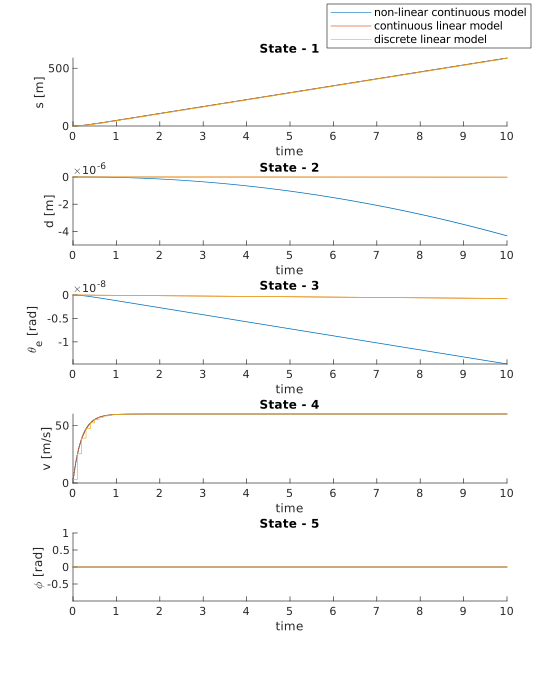
\includegraphics[width=\textwidth]{figures/ex2_states.pdf}
	\subcaption{Applying a step signal on the reference speed $u_1$.}
	\end{subfigure}
	\caption{Experiments in the linear regime of the model. On the left the nominal input is applied and on the right a (rather large) step in the speed is applied. As the system behaves linearly in this setting, the linearization error is very low. Note the small scale on the angle axes.}
	\label{fig:ex1_ex2}
\end{figure}



\section{Case Study Session 2}
\section{Case Study Session 3}

\end{document}
